% *************************************************************************
\chapter[Working title: Quantum Chemistry Based Enzyme Activity Engineering]
{Working title: Quantum Chemistry Based Enzyme Activity Engineering\label{ch1}}
\chapauth{Martin R. Hediger$^{a}$, Harm Otten$^{b}$
\chapaff{$^{a}$Z\"urich\\
$^{b}$K{\o}benhavn\\
m---@---.ch\\
harm.otten@maxlab.lu.se}}
% *************************************************************************


% *************************************************************************
% *************************************************************************
\section{Motivation}\label{sec:mot}
Let us imagine two companies A and B.
Both companies use very similar technical equipment to carry out the biotechnological process $\ce{a}$ $\xrightarrow{Enzyme}$ $\ce{b}$ using two individual versions of the indicated catalyst.
Company A uses an enzyme with a rate constant $k_\text{A} = 1000s^{-1}$ while company B uses an enzyme with $k_\text{B} = 2000s^{-1}$.
Letting all other things be equal, the process of company B will therefore only require half the time to produce one Mole of product compared to the time required for company A.
Company B therefore can save energy required to keep the reaction volume at a certain temperature.
The need for efficient catalysts arises from such an outline and the commercial implications of these considerations are immediate.\footnote{We use the terms \textit{enzme} and \textit{bio-}/\textit{catalyst} interchangeably.}\\
Increasing the performance of enzymes however is still far from trivial and forms a growing body of research.
What is clear though is that the development of such catalysts is costly, in terms of manpower, material and energy -- if carried out in the laboratory.
A number of companies have in fact formed around this demand: Novozymes (DK), Genzyme (US) or DSM (NL) to name but a few\cite{meyer2013use, kirk2002industrial, beilen2002enzyme, schmid2002use}.\\
Laboratory costs can however be saved to a large part if the development is carried out \textit{in silico}.
The proof that computational results are as reliable as experimental results has been provided not too long ago\cite{claeyssens2006high}.
The foundation for successful application of computational enzyme engineering has thus been laid out.
It is therefore natural to ask: Why hasn't this become more important yet?
Why are there not more job openings at pharmaceutical and biotechnology companies looking for computational enzyme engineers?
The field, after all, did receive the Nobel price in Chemistry 2013.\\
By giving an overview and some details in this article, we hope to also, at least in part, answer these questions.
% *************************************************************************


% *************************************************************************
\section{Introduction}\label{sec:intro}
We provide an introduction into the topic of enzyme catalysis modeling for interested people from inside and outside of the field.\\
We outline the latest achievements, methods in use and outline required developments to establish computational enzyme engineering not only in the literature, but also in (commercial) practice.\\
Modeling involving enzymes happens in different forms.
In one form, the enzyme is a constant parameter and the variable is the inhibitor.
These tasks are usually addressed by docking approaches and studies involving millions of substrates have been published\cite{zhou2010high}.
In another form, the substrate is constant but the enzyme can vary.
The approaches to this task, as it appears, are much less established.
The reasons are manifold, primarily it appears that modeling of an enzyme is less straightforward than a small inhibiting molecule.
Again, why is that?

As is known in the community, enzymes behave highly non-predictable.
The best reasoning about a mutation (except for elimination of the catalytic residues) will not even allow to decide \textit{qualitatively} if the mutated enzyme will be more or less active.
Shifts in pH optima might be predicted more readily\cite{ludwiczek2013strategies}.
It is proposed therefore that in cases where no \textit{a priori} knowledge about how an enzyme should be engineered is available, the only reasonable strategy is to carry out systematic screening studies.
For these to be feasible, either the computer power needs to be very large or the method has to be fast, there is an inherent trade off in this situation.
Once initial lead structures are identified, higher level methods can be used to narrow down on most promising candidates.

This review is written for a more general audience.
For specialized details, the reader is referred to the primary literature.
The intention is to provide an accessible introduction into the field of quantum chemical modeling of enzymatic reactions, highlight advantages of using quantum chemistry and also point out points where special care needs to be taken.

Aims of quantum chemical screening assay
\begin{itemize}
\item Fast
\item easy to setup
\item qualitative accuracy
\end{itemize}
% *************************************************************************


% *************************************************************************
% *************************************************************************
\section{Motivation Summary}\label{sec:mot_sum}
Main messages:
\begin{itemize}
\item Screening 317 single and 111 double mutants with av. 29 h per barrier and 1 CPU per interpolation point
\item Correct mechanisms using PM6
\item Barriers in agreement (calc. 18.5, exp. 17.0 kcal/mol)
\item 15/22 correctly predicted (using many approximations and not full model)
\item No bias, more active double mutants identified
\item largely automated
\item For CALB lowest barriers close to WT, BCX lowest barriers lower than WT
\end{itemize}
% *************************************************************************


% *************************************************************************
% *************************************************************************
\section{Methods}\label{sec:methods}
A variety of methods has been established for the use to model enzyme catalysis.
Depending on the properties of interest, the system is treated differently.
Molecular mechanics methods allow to study the structural behavior of the enzyme over a significant time period and provide details about rearrangement of loop motives.
The description of chemical reactivity however requires the description of the electronic structure of the system (molecular mechanics models do not allow the description of bond formation and braking processes).
In this regime, again a number of specialized methods have become available.

\subsection{Idea collection}
Practical applicability of QM based enzyme screening has a couple of problems:
\begin{itemize}
\item The structures of the enzyme in the relevant state of the reaction need to be available, ie. an enzyme-substrate complex (ES) and a transition state (TS) analog (usually an inhibited species)
\item If the mechanism is not established, the reaction can usually follow various pathways -- these would need to be checked in order to find a best guess at the rate determining step
\item Identification of the transition state is difficult and depends intimatly on the structure, optimizing two structures differing by 0.1 \AA in a particular bond length can result in identification or not identification of the TS
\item \textit{Every method has it's chemistry}. The results of one QM chemistry need to be verified, usually high-level standard reference methods are computationally too demanding to be applicable to a large system
\item Modeling software is available, PyMOL, Schr\"odinger, Chem?? (Walter Thiel, commercially) but everything is still very much custom work (especially the data analysis, programs output format is like from last century), this is probably the major reason preventing the use of QM as standard method in industry. Compare docking and MD methods have software which is designed towards user friendlyness and has become established in industry
\item GTKDynamo is an exceptionally good example for what it should look like, unfortunately only small community
\item Many papers claim that ``\textit{future developments are directed at further automating the presented approach}''.
Obviously these remarks are directed at making the method industrially applicable by avoiding the requirement to carry out complicated setup and configuration steps\cite{rathore2013advances}.
In reality, such future developments, to the great unfortune of the whole field, are rarely realized -- speculation on the reasons is beyond the scope of this article.
Nevertheless, almost no publication fails to mention the potential applications in drug design.
\item Computational considerations are only rarely taken into account but greatly help at putting the whole approach into perspective: ``\textit{We do not think that this approach is that relevant for high-throughput screening for several reasons.
First, the amount of calculations required for a single compound is not scalable to thousands or millions of ligands, and second, because the degree of detail provided by the methodology is probably not needed during the screening phase.
Instead, we en- visage a successful application in the lead optimization phase on possible tens of lead compounds to completely reconstruct and understand their binding pathways before moving forward in the pipeline.
The method, although computationally expensive, is certainly feasible if performed on just a few ligands as indicated.
Here, we have made use of our volunteer GPU project GPUGRID.net (7) based on ACEMD (6).
Extrapolating from the current study, it would be possible to reconstruct the binding pathways of 5 to 10 ligands per week in-house on a moderately sized GPU cluster of 32–64 GPUs.}''\cite{buch2011complete}
\end{itemize}

\subsection{Calculation methods}
Different methods used should be briefly described to make it easier for the reader of the literature to understand what is going on
\begin{itemize}
\item AM1/RM1/PM3/PM6/PM7/MOZYME
\item DFT/B3LYP/Dispersion corrections/M06/...
\item Modeling procedures: Define constraints- how does it affect the calculation (examples in literature?)
\item Explain available software: GAMESS, MOPAC
\item Explain parameters of PM6: MOZYME, gradient convergence and NDDO cutoff
\end{itemize}
% *************************************************************************


% *************************************************************************
% *************************************************************************
\section{Applications}\label{sec:apps}

\subsection{General overview}
We have recently presented two studies where new functionality has been introduced into an enzyme active site using quantum chemical methods\cite{10.1371/journal.pone.0049849,hediger2013silico,hediger2013computational}.\\
It is currently agreed that in many cases, rational arguments alone are not sufficient to design new reactivity in an active site.
Put simply, enzymes do not behave in the way the engineer hopes for.
Much rather, the only meaningful strategy proves to be to screen a large number of variant candidates for apparent activity of the desired kind.
In a second step, identified lead candidates are subjected to higher level computational methods and wet-lab experiments which then allow to further establish or dismiss the nature of the candidate.
Given the large mutational space available, initial \textit{in silico} screening has to be efficient.
Hediger \textit{et al.} therefore chose to use semi-empirical methods for the description of the electronic structure of the enzyme-substrate complex.
In their approach, the activities of different variants of an enzyme are ordered by comparing the activation energy required for the rate determining step of the overall reaction -- low activation energies correspond to high anticipated activity of the variant.
Implicitly this assumes high substrate concentration such that $k_\text{cat}$ becomes rate limiting, a reasonable assumption under industrial conditions.

\textbf{General outline of method.}
In both studies, the basic procedure consists of preparing structures for the enzyme substrate complex (``ES'') and the first intermediate (CALB: ``TI''\footnote{Tetrahedral intermediate}, BCX: ``GE''\footnote{\label{foot:ge}Glycosyl enzyme}) and calculating the reaction barrier between these two pairs of structures, respectively.
The reaction barrier is calculated by interpolating between the ES$_\text{CALB}$ and TI or ES$_\text{BCX}$ GE structures, \textit{i.e.} by preparing a set of 10 intermediate structures which approximate the structure of the system along the reaction coordinate.\footnote{In the literature, the terms \textit{interpolation}, \textit{linear transit scan}, \textit{reaction coordinate calculation} or \textit{adiabatic mapping} are frequently used to indicate the same kind of procedure}.
By evaluating the energies for each interpolation frame for the two reactions ES$_\text{CALB}\rightarrow$TI or ES$_\text{BCX}\rightarrow$GE, it becomes possible to obtain an approximate potential energy surface of the reaction, Fig. \ref{fig:calb_reaction}.
The quality of the results of this approach are strongly dependent on how careful the modeling of each of these structures is carried out.
A frequent reason for meaningless results is significant structural rearrangement during the geometry optimization, requiring to interpolate between very different conformations of the two stationary points on each side of the reaction barrier.

\textbf{Requirements.}
The most basic requirements are that a structure representing a bound intermediate along the reaction pathway is available.
Alternatively, a homology model could be used.
Furthermore, ideally the mechanism for the rate determining step is established in the literature.
In case no generally accepted mechanism is reported, a preceeding study could analyse kinetically competing mechanism alternatives.

% *****************************************************************
% Upcoming
\subsubsection{{\textit{Candida antarctica} Lipase B (CALB) Engineering}}
In the studies related to CALB, we answer the question if quantum chemical methods can be used for enzyme activity screening, develop an efficient modeling protocol and verify the calculated predictions with experimental results.
The model system used in this study was CALB and the reaction studied is the hydrolysis of $N$-benzyl-2-chloroacetamide.


\textcolor{blue}{
UPCOMING\\
The questions answered in this study are:
\begin{itemize}
\item Is it possible to screen for mutant activity using quantum chemical methods?
\item Which quantum chemical model can reproduce the accepted mechanism?
\item What are the time requirements depending on the model size?
\item How should the program be configured?
\item What modeling procedure/sequence is needed? Which tools are useful?
\end{itemize}
\begin{figure}[htbp] 
\centering
\begin{minipage}{0.43\linewidth}
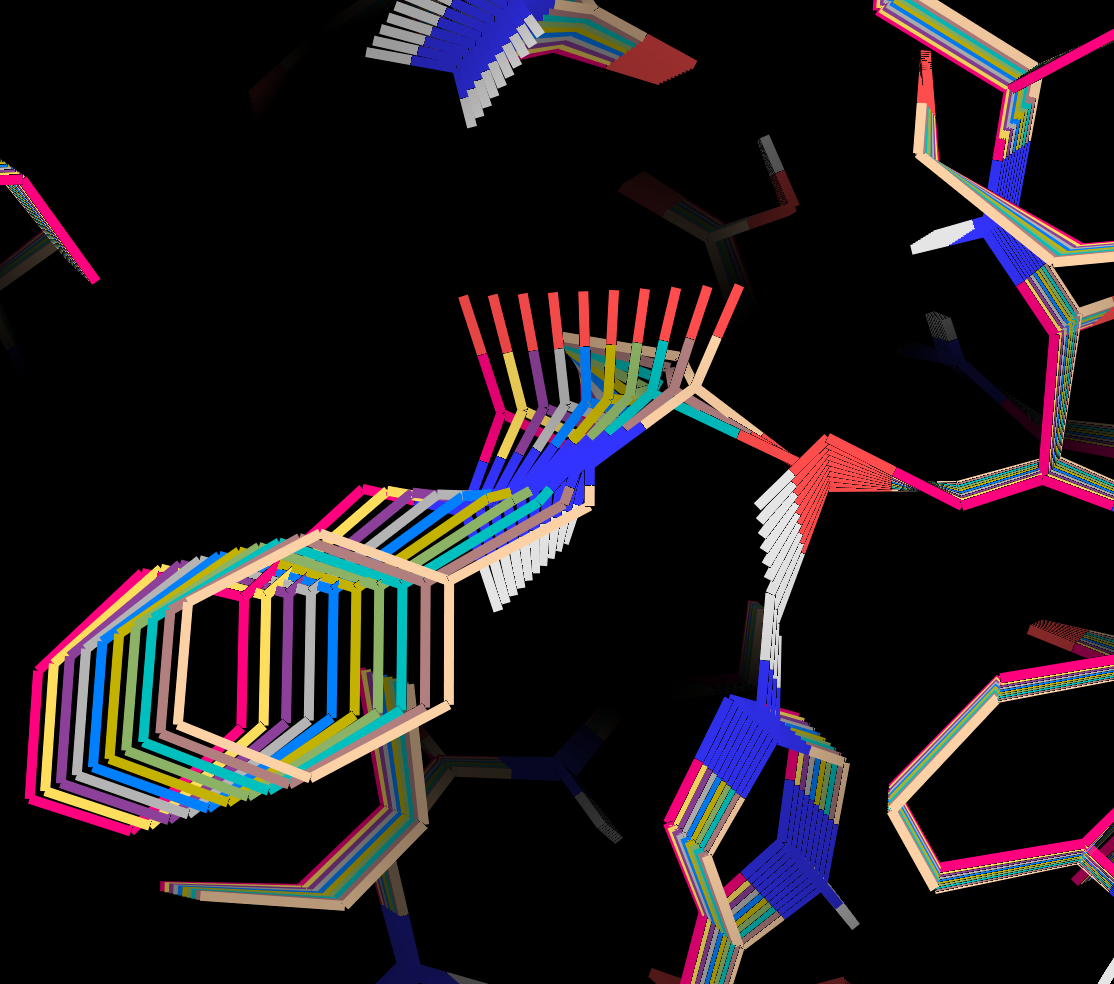
\includegraphics[width=0.90\linewidth]{wt-ini.png}
\end{minipage}
\begin{minipage}{0.55\linewidth}
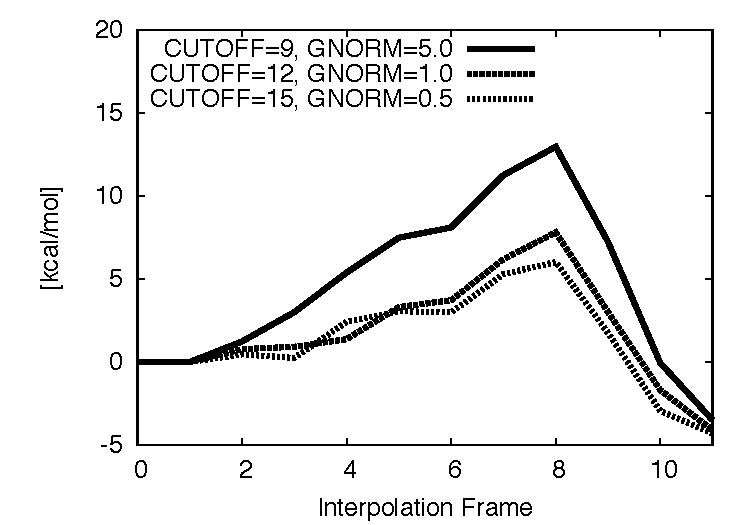
\includegraphics[width=1.00\linewidth]{calb-conv.pdf}
\end{minipage}
\caption{
Intermediate structures along reaction coordinate of CALB reaction.
}
\label{fig:calb_reaction}
\end{figure}
CALB is used as a versatile catalyst in a variety of applications among which enzymatic kinetic resolution of enantiomeric mixtures is of high pharmaceutical importance\cite{gotor2006candida}.
While CALB is also known for its reactive promiscuity\cite{CBIC:CBIC200800318}, if the catalyst can be engineered such as to increase its performance for certain of these applications, possible bottle-necks in production could be widened.\\
About the cutoff: this is only relevant in studies where experimental data for many mutants is available.
Then it can be used to assess the lower barrier for the accuracy.
Given all approximations, x out of y mutants are correctly predicted.
So any method improving on the approximations should provide at least at many correct hits.\\
About the cutoff: this is only relevant in studies where experimental data for many mutants is available.
Then it can be used to assess the lower barrier for the accuracy.
Given all approximations, x out of y mutants are correctly predicted.
So any method improving on the approximations should provide at least at many correct hits.
A number of weak points remain:
\begin{itemize}
\item Selection of model ambiguous/not full structure
\item Not systematically screening all mutants
\item No other protein system/enzymatic reaction tested
\item Binding effects not considered
\item Large rearrangements can not be modeled
\item Semi-empirical methods might not be adequate for metals
\item Subsequent steps of reaction not modeled (eg. product leaving of active site)
\item Different ionization states of residues
\end{itemize}
}

Real world applications of BCX: production of biofuels and papers, CALB: pharmaceutical and fine chemicals[REFS?].
% -----------------------------------------------------------------

\newpage
\subsubsection{\textit{Bacillus circulans} xylanase engineering}
In order to address the points summarized above and to show general applicability of the approach outlined for CALB, the xylanase of \textit{Bacillus circulans} (BCX) is engineered to be catalytically active towards an artifical substrate ($ortho$-nitrophenol-$\beta$-xylobioside), Fig. \ref{fig:substrate}.
\begin{figure}[htbp] 
\centering
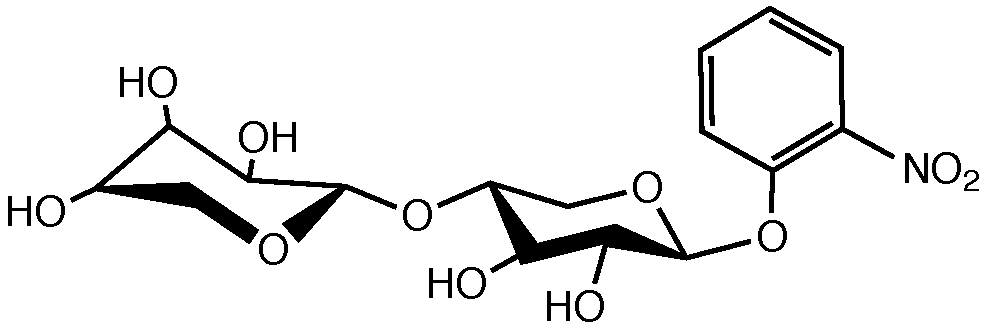
\includegraphics[width=0.85\linewidth]{substrate.pdf}
\caption{
$ortho$-nitrophenol-$\beta$-xylobioside substrate used in BCX study consisting of two xylose units and ONP.
}
\label{fig:substrate}
\end{figure}
In this study, the mechanism was taken from the literature as reported previously\cite{joshi2000hydrogen,joshi2001dissecting}.
In the following, we outline the work reported in the study and illustrate the sequence of simulation and modeling steps.\\
\textbf{WT reaction barrier modeling.}
In a first step, the wild-type (WT) reference reaction barrier is established.
This is a crucial step because all subsequent conclusions about mutants are depending on how good the WT reaction barrier is estimated.
As was done for CALB, only the rate determining step is modeled, Fig. \ref{fig:bcx_mechanism}.
\begin{figure}[htbp] 
\centering
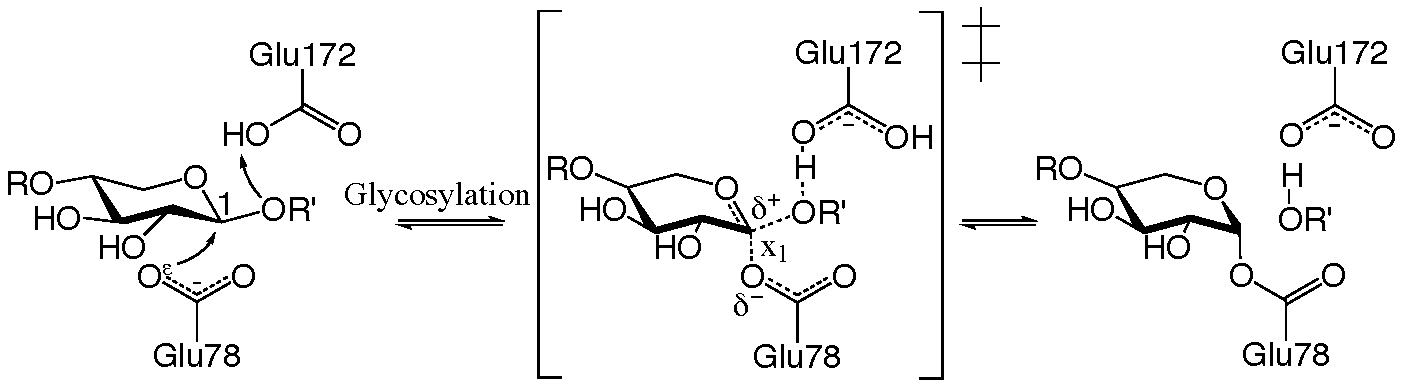
\includegraphics[width=1.0\linewidth]{mechanism.pdf}
\caption{
Rate determining step in conventional glycosylation. $x_1$: constrained reaction coordinate; $R$: xylose; 
$R'$: \textit{ortho}-nitrophenol (ONP).
C$_1$ indicating nucleophilic carbon of first xylose unit\cite{hediger2013computational}.
}
\label{fig:bcx_mechanism}
\end{figure}
As outlined in the methods section, the reaction barrier is mapped out by fixing the reaction coordinate ($x_1$ in Fig. \ref{fig:bcx_mechanism}) at discrete, decrementing values while optimizing the rest of the protein structure.
Since the reaction consists of two concerted events (nucleophilic attack by E78 and proton transfer from E172 to ONP), in principle a two-dimensional potential energy surface could be mapped out to determine the reaction barrier.
However, since proton transfer is associated with a rearrangement of the electronic structure, this reaction coordinate is left unconstrained and is handled solely by the quantum chemical method, \textit{i.e.} the proton is free to transfer from or remain on E172.
Forcing the quantum chemical model to do something it would not if left unconstrained most likely results in an increased reaction barrier and therefore it is advisable to keep the number of constraints as low as possible.\\
A PDB structure comprising a covalently linked inhibitor is available (1BVV) and is used as a starting point for the modeling procedure because it gives a very clear indication of how the substrate is located in the active site.
As shown in Fig. 2 in Hediger \textit{et al.} (2013b), two possible modeling pathways were worked out.
In the first one, the ES complex is prepared from the GE structure \textit{before} the GE structure is optimized (see footnote \ref{foot:ge}).
Alternatively, the GE structure is optimized first and then used as a template for the ES structure.
Within this alternative approach, the preparation of the ES structure then just requires minor modifications of substrate conformation before the structure is optimized.\\
Because in this second approach the ES structure very closely resembles the optimized GE structure, it is possible to concentrate the optimization of the ES structure only on the active site, while the remote part of the enzyme remains fixed at the optimized geometry of the GE structure.
This results in very large gains in computational efficiency, which depend on the layer of residues being optimized around the active site.\footnote{The structural constraints are parameters to the calculation program and are prepared programmatically using a PYMOL script. The way the parameters are submitted to the calculation may vary depending on the software used for calculations.}
Fixing, \textit{i.e.} not reoptimizing an already optimized part of the enzyme however also results in slightly increased energy of the ES structure relative to the fully optimized GE structure and so the reaction barriers will be decreased.
This increase (of ES energy relative to GE) results from multiple minor structural strain forming at the interface between the fixed and optimized layers of the structure.
The observations are summarized in Fig. \ref{fig:bcx_constr_constraint_layers}.
% Panel labels have their own minipages to print on same line
\begin{figure}[htbp] 
\centering
\begin{minipage}{0.42\linewidth}
\textbf{A}
\end{minipage}
\begin{minipage}{0.42\linewidth}
\textbf{B}
\end{minipage}
\begin{minipage}{0.47\linewidth}
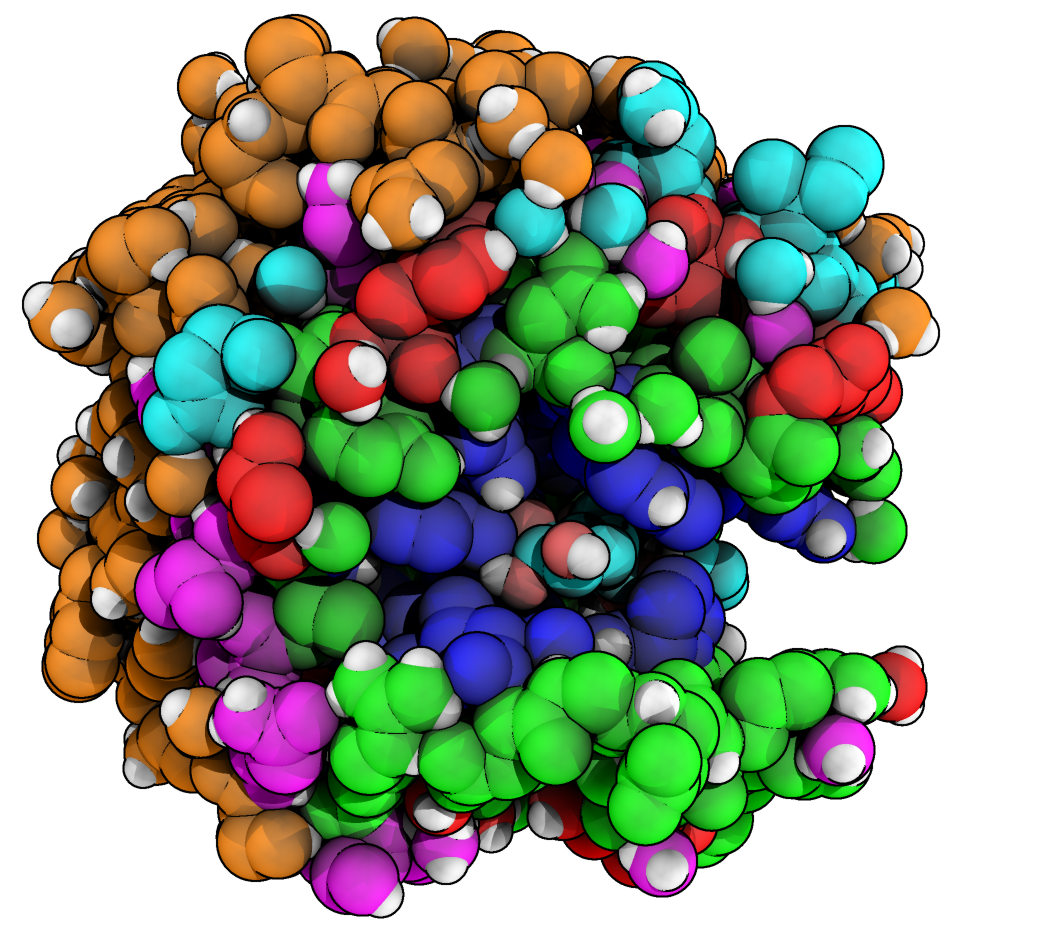
\includegraphics[width=0.95\linewidth]{bcx-constraint-layers-ray-occlusion-2.png}
\end{minipage}
\begin{minipage}{0.51\linewidth}
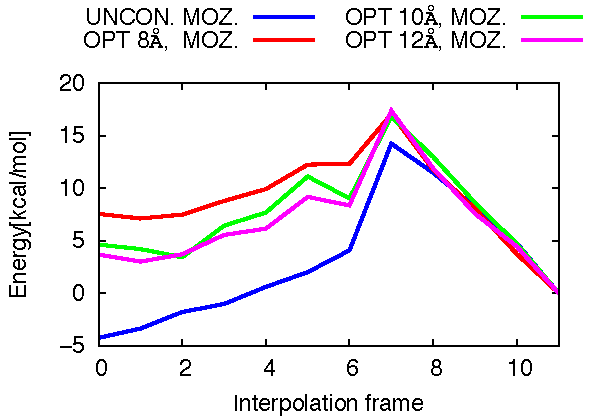
\includegraphics[width=1.00\linewidth]{bcx-barriers-constraint-layers.pdf}
\end{minipage}
\caption{
\textbf{A}: Illustration of optimization layers of BCX with bound ONP substrate.
Color coded residue layers have at least one atom within the indicated distance to any atom of the substrate:
\textit{green} 8 \AA, \textit{red} 10 \AA, \textit{purple} 12 \AA, \textit{cyan} 14 \AA.
\textit{Brown} residues remain at their optimized GE geometry, \textit{dark blue} are residues which are screened for active mutations.
The substrate is visible in the center of the dark blue residues.
\textbf{B}: Calculated reaction barriers for different layers of optimized residues (based on Hediger \textit{et al.} (2013b)).
}
\label{fig:bcx_constr_constraint_layers}
\end{figure}
Based on this second approach, \textit{i.e.} using the optimized GE structure as the template for the ES structure, and when not applying any constraints (apart from the reaction coordinate $x_1$), the reaction barrier is found to be 18.5 kcal/mol which is in very close agreement to the experimentally reported value of 17.0 kcal/mol obtained from transition state theory\cite{joshi2000hydrogen}.
This strongly supports that the outlined modeling procedure, the configuration of the quantum chemical method and the included/omitted physical effects provide a meaningful model of the enzyme kinetics.
As pointed out above, when applying constraints on remote parts of the structure, this can decrease the reaction barrier because the ES structure is increased in energy relative to the GE reference point (which is set to zero).
However, it is reasonable to assume that this relative increase will be the same for all studied structures and so cancels out once mutants are compared relative to each other.  
Overall, application of constraints to remote parts of the enzyme is necessary to reach the desired calculation efficiency of one reaction barrier per day when running each interpolation step in parallel.
Furthermore, application of constraints has been widely adopted by the community\cite{himo2006quantum,siegbahn2009recent,liao2012comparison,lonsdale2013quantum}.
The time required for optimizing the structures with or without constraints are found to differ by a factor of six (Fig. 4B in Hediger \textit{et al.} (2013b)).\\
\textbf{Mutant activity screening.}
By a similar approach as the one outline for the modeling of the WT reaction, it is found that different ways of modeling the set of mutants results in significantly different levels of efficiency, both in terms of required manual efforts as well as in computational time requirements.
We refer to the original publication for details\cite{hediger2013computational} but point out that when, similarly as for the WT, the ES structures of the mutants are based on templates of optimized mutant GE structures, again large gains in computational efficiency are possible (see Fig. 7 in Hediger \textit{et al.} (2013b)).\\
Using PYMOL\cite{PyMOLu}, models of all possible single mutants within a given distance of the substrate are prepared (excluding the catalytically active E78 and E172).\footnote{The PYMOL script used for the preparation of the mutants is available at https://github.com/mzhKU/Enzyme-Screening/blob/master/vsc-bcx.py.}
It is noted that in the current implementation of the presented approach, all mutated side chains are in their default ionization state at physiological pH.
Furthermore, in a number of cases it is not possible to introduce a large side chain in a spatially restricted environment, such cases are discarded.
Lastly, instead of using a side chain rotamer library, each mutated side chain is locally optimized (using an empirical builtin PYMOL function) in the environment of the enzyme before being submitted to the quantum calculation.
This approach allowed to screen a set of 317 single mutants, where on average 29 hours are required to complete the calculations of a full reaction barrier using one CPU for each interpolation point.\footnote{All obtained barriers are provided at http://www.scribd.com/doc/133445214/Supp-Mat-Paper-4.}
From this set of single mutants, for every position $i, j, ...$ in the active site, the mutation resulting in the mutant with the lowest barrier $X_i, Y_j, ...$ is identified.
Then, from this set of single mutants $\{K_l\}$, all possible double mutants $(X_i, Y_j)$ are formed.
Analysis of the reaction barriers of the obtained candidates reveals that the set of double mutants on average has lower activation barriers than the set of single mutants.
Furthermore, the lowest barriers are found among the double mutants.
\begin{figure}[htbp] 
\centering
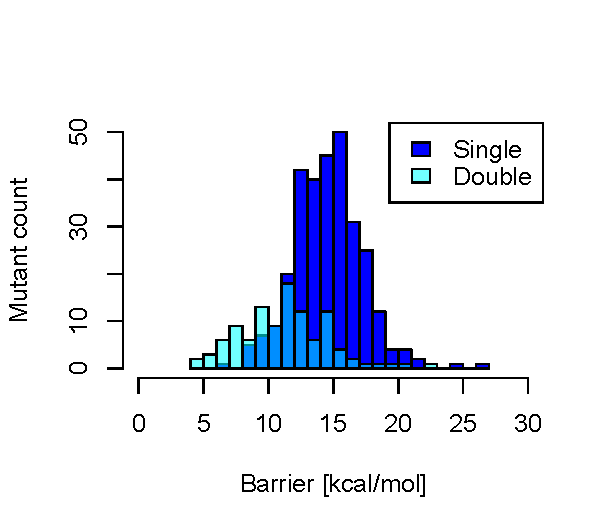
\includegraphics[width=0.95\linewidth]{barrier-distribution.pdf}
\caption{
Barrier distribution of single and double BCX mutants\cite{hediger2013computational}.
The plot is a histogram of reaction barriers, i.e. how many mutants are identified with a given reaction barrier.
}
\label{fig:bcx_barrier_distribution}
\end{figure}
\newline
\textbf{Rationalization of mutants.}
Analysis of the set of mutants indicates that position 127 has strong influence on the activity (9 of 20 best single mutants carry a mutation at that position).
Inspection of the structural arrangement of the Q127W, W9D/E and N35E mutations points to a number of possible explanations of the observed lower barriers, Fig. \ref{fig:bcx_rationalization}.
\begin{figure}[htbp] 
\centering
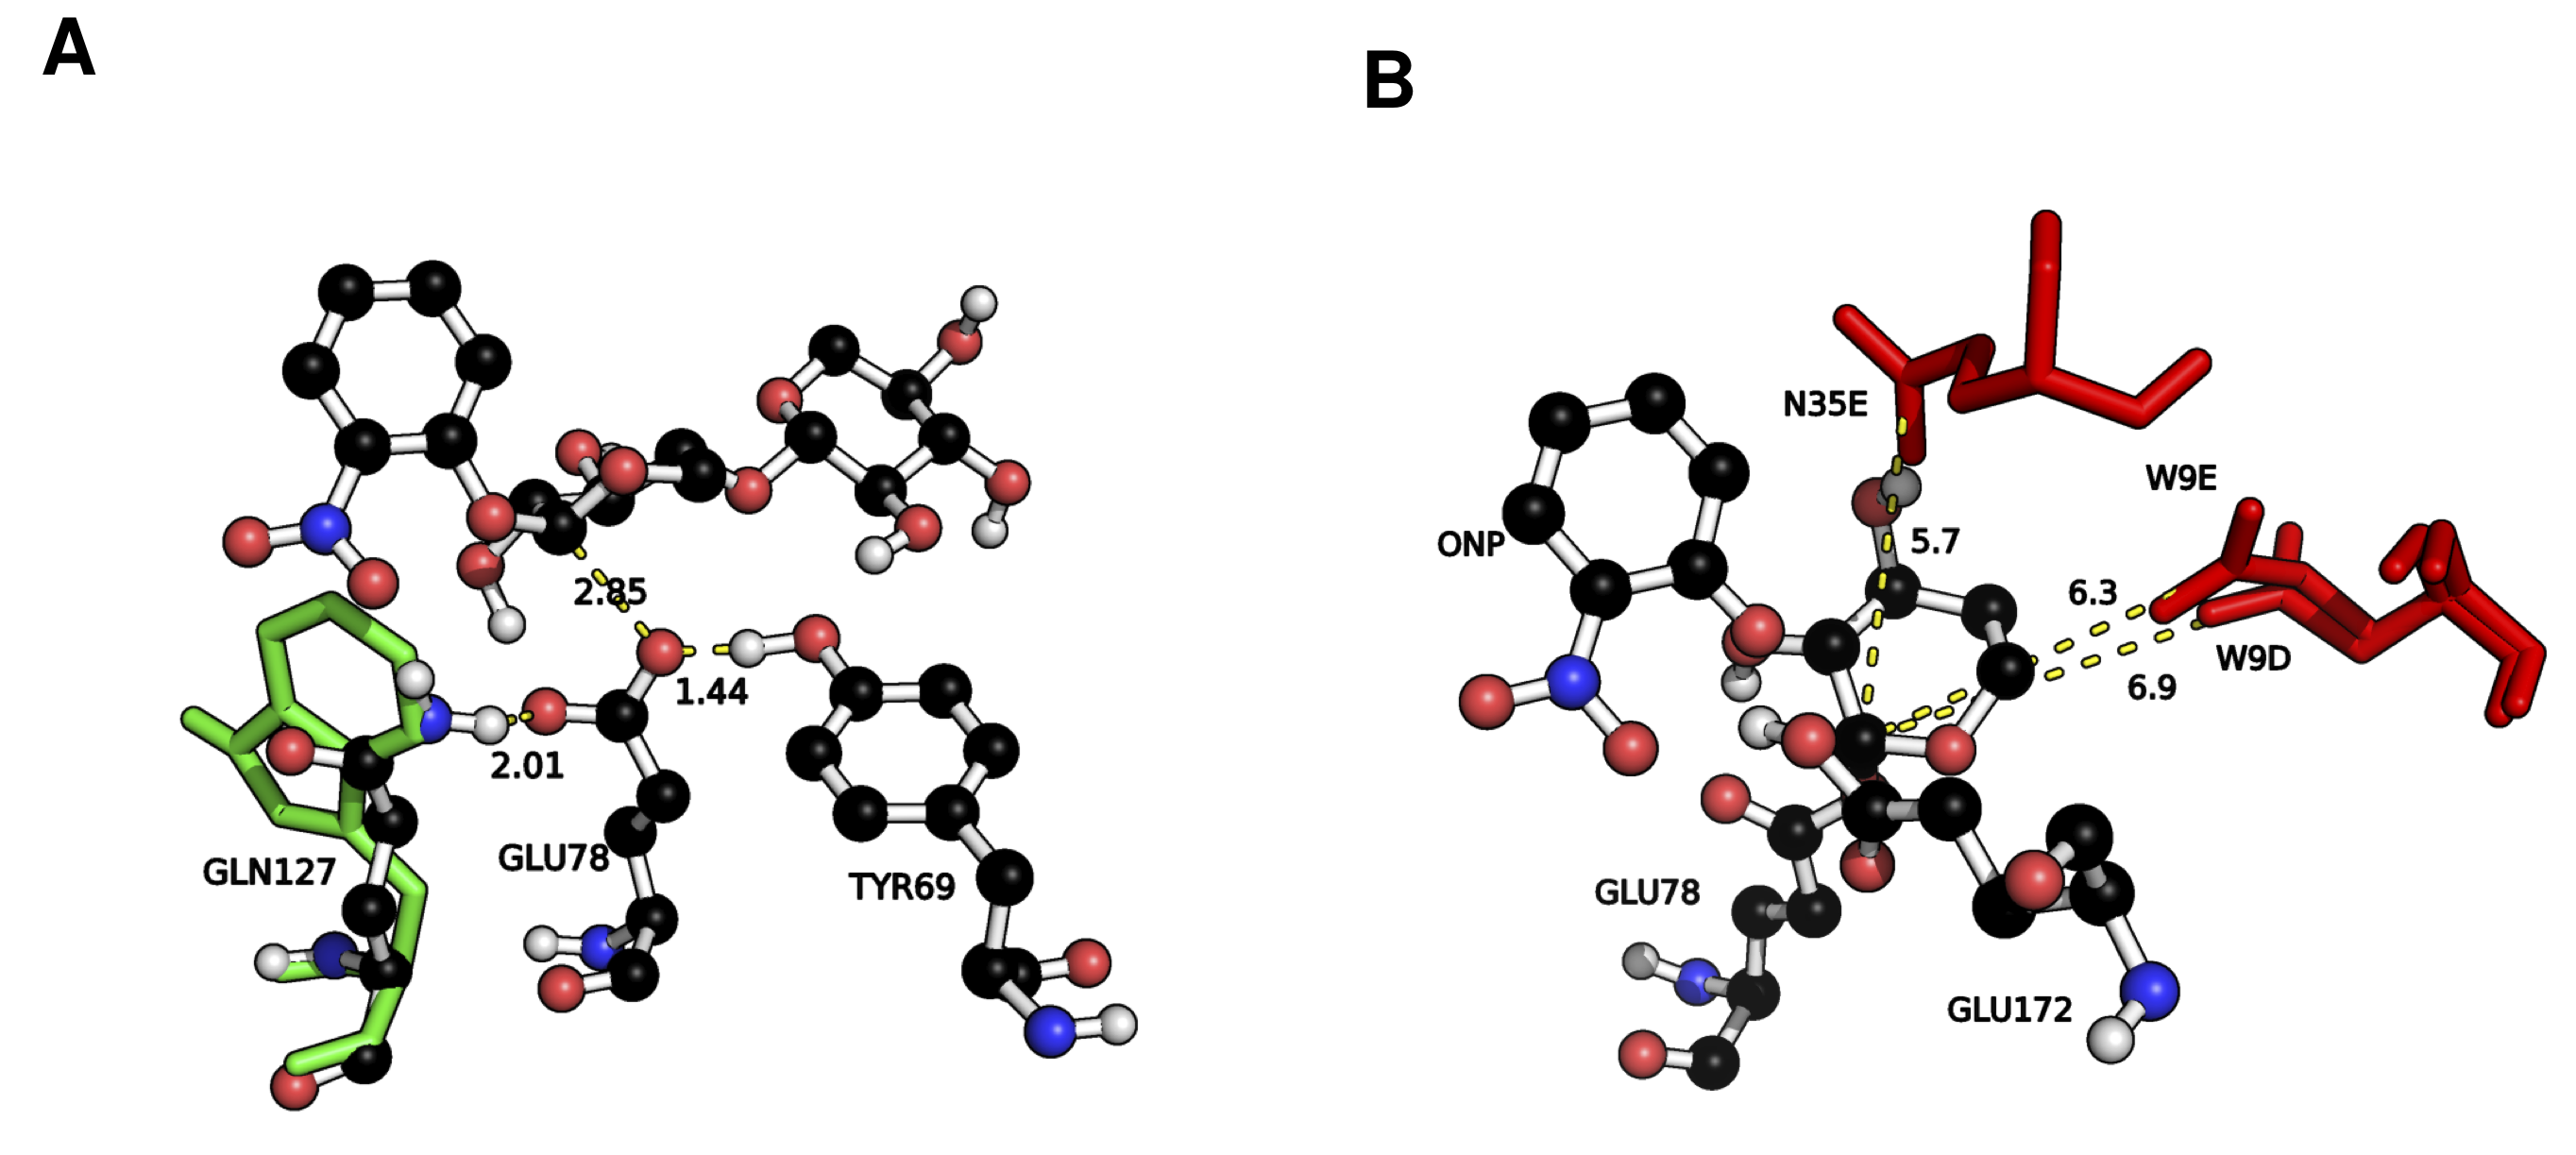
\includegraphics[width=0.99\linewidth]{analyse-charge.png}
\caption{
Rationalization of reaction barriers.
\textbf{A} Overlay of WT (black carbon spheres) and Q127W side-chain (green).
\textbf{B} Stabilizing, coulombic interactions between negative W9D/E or N35E (red) with the nucleophilic, partially positively charged C$_1$ of the substrate.
Distances in \AA\cite{hediger2013computational}.
}
\label{fig:bcx_rationalization}
\end{figure}
As discussed above, the mechanism is postulated to involve a catalytically active, negatively charged E78 residue as the nucleophile.
If Q127 stabilizes the negative charge by hydrogen bonding, the nucleophilic character of E78 is reduced.
Replacing the potential hydrogen bond donor Q127 with a non-hydrogen bonding substitute that can preserve overall structural integrity with a side chain of similar size, such as Q127W, could result in increased nucleophilicity of E78, Fig. \ref{fig:bcx_rationalization} A.
Furthermore, as illustrated in Fig. \ref{fig:bcx_mechanism}, the transition state involves a partially positive charge on C$_1$ of the substrate.
Negative charges on side chains (such as in W9D/E) could act as stabilizers of this negative charge and increase catalytic activity in doing so, \textit{i.e.} by stabilization of the transition state.
Similaryl, when ionized, N35E could act in stabilizing C$_1$ but when in neutral protonation state, it could be acting as a hydrogen bond donor to the catalytically active E172.
This rationalization of N35 mutations would be related to a recently proposed \textit{reverse protonation} mechanism\cite{joshi2000hydrogen}, which still is the subject of ongoing research.

\newpage
\subsection{Interesting QM/MM applications}
\textbf{The cocaine hydrolase guys}\\
Make a cocaine hydrolase better\cite{gao2006computational}.

\subsection{Requirements for advancement of methods}
Experimental catalytic data ($k_\text{cat}$) of many mutants to validate against.
% *************************************************************************


% *************************************************************************
% *************************************************************************
\section{Conclusions}\label{sec:conclusions}

\subsection{Advantages/Disadvantages of using quantum chemistry for modeling enzymatic reactions}
\begin{itemize}
\item Bond formation/breaking can be modeled
\item Large systems might require constraints to reach convergence
\item Calculation times depend strongly on model chemistry used
\item Not yet as established and convenient to use like e.g. docking software
\end{itemize}
